\documentclass[11pt]{scrartcl}
\usepackage{graphicx}
\graphicspath{{./}}
\usepackage[sexy]{evan}
\usepackage[normalem]{ulem}
\usepackage{hyperref}
\usepackage{mathtools}
\hypersetup{
    colorlinks=true,
    linkcolor=blue,
    filecolor=magenta,      
    urlcolor=cyan,
    pdfpagemode=FullScreen,
    }
\usepackage[most]{tcolorbox}
\newcommand{\siku}[4][.21cm]
	{
	\coordinate (tempa) at ($(#3)!#1!(#2)$);
	\coordinate (tempb) at ($(#3)!#1!(#4)$);
	\coordinate (tempc) at ($(tempa)!0.5!(tempb)$);%midpoint
	\draw[black] (tempa) -- ($(#3)!2!(tempc)$) -- (tempb);
	}
	\usetikzlibrary{calc,positioning,intersections} %----------
\renewcommand{\dangle}{\measuredangle}

\renewcommand{\baselinestretch}{1.5}

\addtolength{\oddsidemargin}{-0.4in}
\addtolength{\evensidemargin}{-0.4in}
\addtolength{\textwidth}{0.8in}
% \addtolength{\topmargin}{-0.2in}
% \addtolength{\textheight}{1in} 


\setlength{\parindent}{0pt}

\usepackage{pgfplots}
\pgfplotsset{compat=1.15}
\usepackage{mathrsfs}
\usetikzlibrary{arrows}

\title{Pythagoras Theorem}
\author{Azzam Labib (IG: haxuv.world)}
\date{G3-4 | 30 May 2024}
\begin{document}
\maketitle
\section{Formula}
One of the math formula that became very popular among us (and so popular in pop culture). Given a right triangle $ABC$ where $C$ is a right angle ($\angle C = 90^\circ$).\\

If the sides length $AB=c$, $BC=a$, and $CA=b$, then
\begin{align*}
    a^2+b^2=c^2
\end{align*}
\begin{center}
\begin{tikzpicture}[scale=1.5]

% titik-titik segitiga
\coordinate[label=left:$C$] (C) at (-1.5cm,-1.cm);
\coordinate[label=above:$B$] (B) at (-1.5cm,1.8cm);
\coordinate[label=right:$A$] (A) at (0.5cm,-1.cm);

% pembuatan segitiga
\draw (A) -- node[right]{$c$} (B) -- node[left]{$a$} (C) -- node[below]{$b$} cycle;

% right angle marker at C
\siku[10pt]{A}{C}{B}

\end{tikzpicture}
\end{center}

\section{Example}
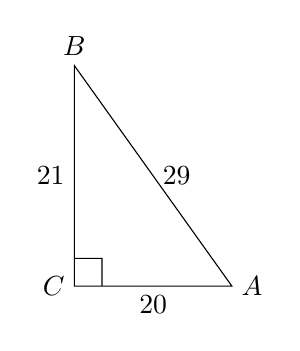
\begin{tikzpicture}

% titik-titik segitiga
\coordinate[label=left:$C$] (C) at (-1.5cm,-1.cm);
\coordinate[label=above:$B$] (B) at (-1.5cm,1.8cm);
\coordinate[label=right:$A$] (A) at (0.5cm,-1.cm);

% pembuatan segitiga
\draw (A) -- node[right]{$29$} (B) -- node[left]{$21$} (C) -- node[below]{$20$} cycle;

% right angle marker at C
\siku[10pt]{A}{C}{B}

\end{tikzpicture}
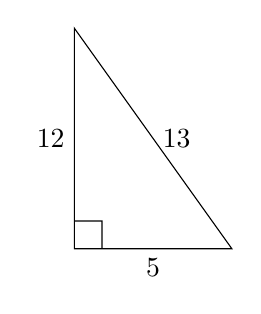
\begin{tikzpicture}

% titik-titik segitiga
\coordinate (C) at (-1.5cm,-1.cm);
\coordinate (B) at (-1.5cm,1.8cm);
\coordinate (A) at (0.5cm,-1.cm);

% pembuatan segitiga
\draw (A) -- node[right]{$13$} (B) -- node[left]{$12$} (C) -- node[below]{$5$} cycle;

% right angle marker at C
\siku[10pt]{A}{C}{B}

\end{tikzpicture}
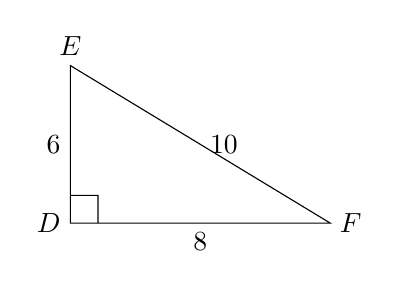
\begin{tikzpicture}

% titik-titik segitiga
\coordinate[label=left:$D$] (C) at (-1.5cm,-1.cm);
\coordinate[label=above:$E$] (B) at (-1.5cm,1cm);
\coordinate[label=right:$F$] (A) at (1.8cm,-1.cm);

% pembuatan segitiga
\draw (A) -- node[right]{$10$} (B) -- node[left]{$6$} (C) -- node[below]{$8$} cycle;

% right angle marker at C
\siku[10pt]{A}{C}{B}

\end{tikzpicture}
\end{document}


